% --------------------------------------
% Chapter 7 Solutions
% --------------------------------------


\subsection{7.1 $\bigstar$}
This basically stems from the fact that integrating $z^{n}$ will give $\frac{1}{n+1}z^{n+1}$, when $n\neq -1$. But the function $f(z)=z^{n+1}$ is not multivalued, thus the integral must vanish.\\ \\ To see this explicitly, suppose $z'$ is $z$ rotated by $2\pi$, i.e $z'=z\cdot e^{2i\pi}$. Then $(z')^{(n+1)}=z^{n+1}\cdot e^{2i\pi(n+1)}=z^{n+1}$. Hence
$$\int_{z}^{z'}z^n\, dz=\oint z^n\, dz=\frac{1}{n+1}(z')^{n+1}-\frac{1}{n+1}z^{n+1}=0$$


\subsection*{7.2 $\bigstar$}
It is easy to see once we note that $\oint z^n\, dz=0$ for all $n\neq -1$, which we showed in Question 7.1. \\ \\
The Maclaurin expansion of $f(z)$ is $f(z)=\sum_{k=0}^{\infty}\frac{f^{(k)(0)}}{k!}z^k$. Thus
\begin{align*}
\frac{n!}{2\pi i}\oint \frac{f(z)}{z^{n+1}}\, dz&= \frac{n!}{2\pi i}\oint \frac{\sum_{k=0}^{\infty}\frac{f^{(k)}(0)}{k!}z^k}{z^{n+1}}\, dz\\
&= \frac{n!}{2\pi i}\sum_{k=0}^{\infty}\frac{f^{(k)}(0)}{k!}\oint z^{k-n-1}\, dz\\
&=0+0+\ldots +\frac{f^{(n)}(0)}{2\pi i}\oint z^{-1}\, dz+0+0+\ldots\\
&=\frac{f^{(n)}(0)}{2\pi i}\cdot 2\pi i\\
&=f^{(n)}(0)
\end{align*}


\subsection{7.4 $\bigstar\bigstar$}
We will consider the case with 3 poles. First, we note that we can always deform the contour so that we can have closed contours around each of the poles. Each circle contains only one pole. Hence the total integral will be the sum of each of the closed circle integrals.\\ \\
Now we need to evaluate the circular integrals. So let us consider the circle around the pole $a_1$. We have that $h(z)$ is analytic within the contour, hence we can express it as a Taylor series about $a_1$, i.e  $h(z)=\sum_{k=0}^{\infty}\frac{h^{(k)}(a_1)}{k!}(z-a_1)^k$
Thus 
\begin{align*}
f(z)&=\frac{1}{(z-a_1)^n}\sum_{k=0}^{\infty}\frac{h^{(k)}(a_1)}{k!}(z-a_1)^k=\sum_{k=0}^{\infty}\frac{h^{(k)}(a_1)}{k!}(z-a_1)^{k-n}
\end{align*}
Now we have from question [7.1] that $\oint z^n\, dz=0$ for all $n\neq -1$. It is easy to see that the same must be true for $(z+p)^n$. So the closed-integral of $(z-a_1)^{k-n}$ is only non-zero for $k-n=-1 \implies k=n-1$. Thus 
\begin{align*}
\oint_{\gamma_1} f(z)\ dz&=\oint_{\gamma_1} \sum_{k=0}^{\infty}\frac{h^{(k)}(a_1)}{k!}(z-a_1)^{k-n}\ dz\\
&=\sum_{k=0}^{\infty}\frac{h^{(k)}(a_1)}{k!}\oint_{\gamma_1} (z-a_1)^{k-n}\ dz\\
&=\frac{h^{(n-1)}(a_1)}{(n-1)!}\oint_{\gamma_1} (z-a_1)^{-1}\ dz\\
&=\text{Res}[f(z),a_1]\cdot 2\pi i
\end{align*}
as we are given that $\frac{h^{(n-1)}(a_1)}{(n-1)!}=\text{Res}[f(z),a_1]$. Thus the total integral is (the sum of the residues at the poles)$\times 2\pi i$.


\subsection{7.5 $\bigstar\bigstar\bigstar$}
\textbf{Question:} \ Show that
$$\int^{\infty}_{0}x^{-1}\sin x=\frac{\pi}{2}$$
\textbf{Strategy:} Penrose recommends we consider the function $f(z)=z^{-1} e^{iz}$ instead of the obvious $z^{-1} \sin z$.\footnote{The reason for this is that the integral of $z^{-1} \sin z$ around the semicircle $\Gamma_1$ does not go to 0 as $R\to\infty$. It is much easier showing things go to zero than explicity evaluating them, and so we avoid this difficulty by integrating around $z^{-1} e^{iz}$ instead.}   We integrate along the contour in \textbf{Fig. 1}. We can easily find the value of the total integral using the Cauchy formula, $\oint f(z)z^{-1}\, \text{d}z=2\pi i\cdot f(0)$ (Road TR pg 127). We can then calculate the contribution from $\Gamma_2$ as $\epsilon\to 0$, and we will show that as $R\to \infty$, $\Gamma_1\to 0$. Then the contribution from the real axis plus $\Gamma_2$ equals what we got using the Caucy formula. Thus we can get the value of the integral along the real axis. Finally, we know that the original integral is just the imaginary part of the integral of $z^{-1} e^{iz}$.\\ \\
\begin{figure}\label{e}
\includegraphics[scale=0.8]{chapters/images/7.5.eps}
\caption{The contour along which we integrate $f(z)=z^{-1} e^{iz}$, with the star indicating the singularity at the origin.  }
\end{figure}  
\textbf{Solution:} Making use of the Cauchy formula, and that in general $z=x+iy$ so $z=x$ on the real-axis,
\begin{align*}
\oint_\Gamma z^{-1}e^{iz} \ dz &= 2\pi i e^{i\cdot 0}=2\pi i\\
&=\int_{\Gamma_1} z^{-1}e^{iz}\ dz+\int_{\Gamma_2} z^{-1}e^{iz}\ dz+\int_{-R}^{-\epsilon} x^{-1}e^{ix}\ dx+\int^{R}_{\epsilon} x^{-1}e^{ix}\ dx
\end{align*}
It turns out that 
$$\lim_{R\to \infty}\int_{\Gamma_1} z^{-1}e^{iz}\ dz =0$$
This is difficult to show directly. It is easiest making use of a result not given in the Road TR, known as \emph{Jordan's lemma}. The statement (and simple proof) of the Lemma is given in the Appendix, from which it is easy to see that this result follows.\footnote{This may seem as cheating, but the method of the proof could be used to directly get the result. Why not just get the general result instead?} \\ \\
Now we want to find the value of the integral along $\Gamma_2$ as $\epsilon\to 0$. We give two different ways of getting this.
\subsection*{Evaluating $\Gamma_2$, method 1}
\begin{align*}
\lim_{\epsilon \to 0} \int_{\Gamma_2} z^{-1}e^{iz}\, dz&=\lim_{\epsilon \to 0} \int_{\Gamma_2} z^{-1}\left[ 1+\frac{1}{1!}(iz)+\frac{1}{2!}(iz)^2+\ldots\right ]dz\\
&=\lim_{\epsilon \to 0} \int_{\Gamma_2} z^{-1}\ dz+\lim_{\epsilon \to 0} i\int_{\Gamma_2} dz-\lim_{\epsilon \to 0} \frac{1}{2}\int_{\Gamma_2} z \ dz+\ldots
\end{align*} 
But $\lim_{\epsilon \to 0} \int_{\Gamma_2} z^{n}\ dz=0$
for all $n\geq 0$.\footnote{The maximum value of $z^n$ on $\Gamma_2$ goes to 0 as $\epsilon \to 0$, and the length of  $\Gamma_2$ also goes to zero. Hence the integral must also go to zero.} Hence 
$$ \lim_{\epsilon \to 0} \int_{\Gamma_2} z^{-1}e^{iz}\, dz=\lim_{\epsilon \to 0} \int_{\Gamma_2} z^{-1}\ dz$$
 Now we know that $z=\epsilon e^{i\phi}$. Hence 
$$d z=i \epsilon e^{i\phi}d\phi$$
Thus 
\begin{align*}
\lim_{\epsilon \to 0} \int_{\Gamma_2} z^{-1}\ dz&=\lim_{\epsilon \to 0} \int^{0}_{-\pi} \frac{1}{\epsilon e^{i\phi}}i \epsilon e^{i\phi}d\phi \\
&=i\lim_{\epsilon \to 0} \int^{0}_{-\pi} d\phi =i\pi \\
\end{align*}
\subsection*{Evaluating $\Gamma_2$, method 2}
The result can be obtained using only Cauchy's formula, and symmetry. We do this here. So using Eulers formula, we have that 
\begin{align*}
 \int_{\Gamma_2} z^{-1}e^{iz}\, dz&= \int_{\Gamma_2} z^{-1}\cos z\, dz+i \int_{\Gamma_2} z^{-1}\sin z\, dz
\end{align*}
Now suppose we chose to integrate around a complete circle centred on $z=0$. In this case, we can use Cauchy's formula:
\begin{align*}
 \oint z^{-1}\cos z\, dz+i \oint z^{-1}\sin z\, dz&=2\pi i \cos(0)+2\pi i \cdot i \sin (0)\\
&=2 \pi i+0
\end{align*}
The circle consists of two semicircles, $\Gamma_2$ and, let us call the other $\phi$. Now $\Gamma_2$ is evaluated from $z=-\epsilon$ to $z=\epsilon$, then let $\phi$ be evaluated from $z=\epsilon$ to $z=-\epsilon$. Now as $f(z)=z^{-1}\sin z$ is a symmetric, i.e $f(-z)=f(z)$, we have that $$\int_{\Gamma_2} z^{-1}\sin z\, dz= \int_{\phi} z^{-1}\sin z\, dz$$
Hence 
$$\oint z^{-1}\sin z\, dz=\int_{\Gamma_2} z^{-1}\sin z\, dz+ \int_{\phi} z^{-1}\sin z\, dz=2 \int_{\Gamma_2} z^{-1}\sin z\, dz=0$$
Next, we note that $z^{-1}\cos z$ is antisymmetric, and hence 
$$\int_{\Gamma_2} z^{-1}\cos z\, dz=- \int_{\phi} z^{-1}\cos z\, dz$$ 
Hence $\int_{\Gamma_2} z^{-1}\cos z\, dz=\pi i$ and so $\int_{\Gamma_2} z^{-1}e^{iz} \, dz=\pi i$.\\ \\
Putting the contributions to all the paths together, and noting that
$$\int_{-R}^{-\epsilon} x^{-1}e^{ix}\ dx=\int^{R}_{\epsilon} x^{-1}e^{ix}\ dx,$$
we get that
\begin{align*}
\oint_\Gamma z^{-1}e^{iz} \ dz &=2i\pi \\
&=0+i\pi+2\lim_{\frac{1}{R},\epsilon\to 0}\int^{R}_{\epsilon} x^{-1}e^{ix}\ dx\\
&=i\pi+2\int^{\infty}_{0} x^{-1}e^{ix}\ dx\\
\implies  \ \ \ \ \ \ \ &\int^{\infty}_{0} x^{-1}e^{ix}\ dx =i\frac{\pi}{2} \\
\implies  \ \ \ \ \ \ \ &\int^{\infty}_{0} x^{-1}\cos x\ dx+i\int^{\infty}_{0} x^{-1}\sin x\ dx =i\frac{\pi}{2}
\end{align*}
This implies that $\int^{\infty}_{0} x^{-1}\cos x\ dx=0$, as it is real and the real part of $i\frac{\pi}{2}$ is 0. Hence
$$\int^{\infty}_{0} x^{-1}\sin x\ dx =\frac{\pi}{2}$$


\subsection{7.6 $\bigstar\bigstar \bigstar$}
Let $$f(z)=z^{-2}\cot z\pi=z^{-2}\cos z\pi(\sin z\pi)^{-1}$$
We integrate about the square contour $\Gamma$ as shown in \textbf{Fig. 2}. We know from question [7.4] that this integral will equal the sum of the residues within the contour. Hence
\begin{equation}\label{totalint}
\frac{1}{2\pi i}\oint_\Gamma f(z)=\text{Res}[f(z),0]+\sum^{-1}_{n=-N}\text{Res}[f(z),n]+\sum^{N}_{n=1}\text{Res}[f(z),n]\end{equation}
Let us investigate the residues. The function $f(z)$ has a pole at $z=0$ and whenever $\sin \pi z=0$, which will be when $z=n$, $n\in \mathbb{Z}$. Penrose recommends that we use the results of [7.4]. In order to use the formula for the residue, we need to know what order pole we dealing with. At $z=0$, $(\sin \pi z)^{-1}$ has a pole of order 1 also. One can easily see this from the series $(\sin \pi z)^{-1}=(\pi z-\frac{(\pi z)^3}{3!}+\ldots)^{-1}=(\pi z)^{-1}(1-\frac{(\pi z)^2}{3!}+\ldots)^{-1}=(\pi z)^{-1} g(z)$, where $g(z)$ is obviously regular at $z=0$. As $\cos \pi z= 1+\ldots$, we have that the pole of $f(z)$ at $z=3$ is of order 3. The other poles at $z=n$, $n\neq 0$ are obviously of order 1.\footnote{This is not obvious from the series, but due to the periodicity of $\sin z$, if the pole at $z=0$ is order 1, then the others must be too. This is because $\sin(\pi n)=\pm \sin(0)$ (depending on $n$ even or odd), so has order 1.}\\ \\
Lets find the residue at $z=0$. To do this, first note that we can write $f(z)=z^{-3}h(z)$ where $h(z)=z\cot \pi z$, and is regular around $z=0$. Also,\footnote{This is easy to find using the Quotient rule on pg. 115 RTR, and won't bother showing it here.}
$\frac{d }{d z}\cot \pi z=\frac{\pi}{\sin^2(\pi z)}=\pi \csc^2(\pi z)$
Then from [7.4], we have that 
\begin{align*}
\text{Res}[f(z),0]&=\lim_{z\to 0}\left[\frac{1}{2!}\frac{d^2 h(z)}{d z^2}\right]=\lim_{z\to 0}\left[2\pi^2 z \cos(\pi z) \csc^3(\pi z)-2\pi\csc^2(\pi z)\right]\\
&=\lim_{z\to 0}\left[  \pi^2 z \cos(\pi z) -\pi\sin(\pi z)            \right]\csc^3(\pi z)\\
&=\lim_{z\to 0}\pi\cdot\left[ \pi z(1-\frac{(\pi z)^2}{2!}+\ldots)-(\pi z -\frac{(\pi z)^3}{3!}+\ldots)\right]\frac{1}{(\pi z)^3}\cdot \frac{1}{(1+\ldots)^{3}}\\
&=\lim_{z\to 0}\pi\cdot\left[-\frac{(\pi z)^3}{3}+\ldots\right]\frac{1}{(\pi z)^3}\cdot \frac{1}{(1+\ldots)^{3}}\\
&=-\frac{\pi}{3}
\end{align*}
Now we find the residue at $z=n$, $n\neq 0$. As the pole is of order 1, we can write $f(z)=(z-n)^{-1}k(z)$ where $k(z)=z^{-2}(z-n)\cot \pi z$ is regular around $z=n$. Then 
\begin{align*}
\text{Res}[f(z),n]&=\lim_{z\to n} \frac{k(z)}{0!}=n^{-2}\lim_{x\to 0}x\cdot\cot \pi(x+n) \\
&=n^{-2}\lim_{x\to 0}x\cdot\cot \pi x \\
&=n^{-2}\lim_{x\to 0}\frac{x}{\sin \pi x}\\
&=\frac{1}{\pi n^2}
\end{align*}
where we used $x=z-n$, and the last limit was evaluated using the same argument as used previously for $z=0$. We also used the fact that $\cot(x+\pi n)=\cot x$.\\ \\
Putting all this into \eqref{totalint}, we get
\begin{equation}\label{doubletrouble}
\frac{1}{2 i}\oint_\Gamma f(z)\, dz=-\frac{\pi^2}{3}+\sum^{-1}_{n=-N}\frac{1}{ n^2}+\sum^{N}_{n=1}\frac{1}{ n^2}\end{equation}
We can simplify the above by noting that $\sum^{-1}_{n=-N}n^{-2}=\sum^{N}_{n=1}n^{-2}$.\\ \\ We now show that the total integral vanishes when $N\to\infty$.\footnote{We are working towards an answer (that $1+\frac{1}{2^2}+\frac{1}{3^2}+\ldots=\frac{\pi^2}{6}$), and we can easily see from the above equation that for this answer to be correct, the integral must vanish! Not that for some editions of the book, there is a typo, with Penrose telling us the sum equals $\frac{\pi}{6}$ instead of $\frac{\pi^2}{6}$. } We will make use of the fact that 
$$\left|\oint_\Gamma f(z)\, dz\right|\leq L\cdot \text{max}(|f(\Gamma)|)$$
where $L$ is the length of the contour $\Gamma$.\footnote{This is not given by Penrose, but is pretty obvious.} If $L\cdot \text{max}(|f(\Gamma)|)\to 0$ as $N\to\infty$, then the integral must vanish. Now the length of the square-contour is simple $L=4\cdot (2N+1)=8N+4$. \\
We have $|f(z)|=|z^{-2}\cot \pi z|=|z^{-2}|\cdot|\cot \pi z|$. Obviously $|z|>N$, and so $|z^{-2}|<N^{-2}$. Let us look at the $\cot\pi z$ term. 
\begin{equation*}
|\cot \pi z|=\left|\frac{e^{i\pi z}+e^{-i\pi z}}{e^{i\pi z}-e^{-i\pi z}}\right|=\left|\frac{1+e^{-2i\pi z}}{1-e^{-2i\pi z}}\right|
\end{equation*}
For the vertical sides of the square, $z=\pm(N+0.5)+iy$. For this side, and making use of $e^{\pm 2i\pi(N+0.5)}=-1$,
\begin{align*}
|\cot \pi z|=\left|\frac{1+e^{-2i\pi(\pm N\pm 0.5+iy) }}{1-e^{-2i\pi (N+0.5+iy)}}\right|&=\left|\frac{1-e^{2\pi y}}{1+e^{2\pi y}}\right|\\
&=\left|1-\frac{2}{1+e^{2\pi y}}\right|\leq 1
\end{align*}
For the horizontal sides, $z=x+iy$ with $y=\pm N+0.5$. Using\footnote{These inequalities follow very simply from the geometry of complex numbers.} $\text{max}(|z|,|a|)-\text{min}(|z|,|a|)=\left| |z|-|a|\right|\leq |z+a|\leq |z|+|a|$ and that $|e^{-2i\pi z}|=e^{2\pi y}$,
\begin{align*}
|\cot \pi z|=\frac{|1|+|e^{-2i\pi z}|}{\left| |1|-|e^{-2i\pi z}|\right|}&=\frac{1+e^{2\pi y}}{\left| 1-e^{2\pi y }\right|}\\
&\leq\left|1+\frac{2}{ e^{2\pi y }-1}\right|
\end{align*}
For large $y$, this above tends to $1$, and diverges only for $y=0$. Hence we can find some $k\in \mathbb{R}$, such that for any $N$, $|\cot \pi z|\leq \left|1+2( e^{2\pi y }-1)^{-1}\right|\leq k$
\begin{align*}
\lim_{N\to\infty}\left|\oint_\Gamma z^{-2}\cot\pi z\, dz\right|\leq \lim_{N\to\infty}(8N+4)\cdot |N^{-2}|\cdot k=0
\end{align*}
Hence the integral vanishes as $N\to \infty$. Thus, from \eqref{doubletrouble} we have
\begin{align*}
0&=-\frac{\pi^2}{3}+2\sum^{N}_{n=1}\frac{1}{ n^2}\\
\implies  \ \ \ \ \ \sum^{N}_{n=1}\frac{1}{ n^2}&=\frac{\pi^2}{6}
\end{align*}


\subsection{7.7 $\bigstar\bigstar$}
One way is by recognising $1/z$ to be an incipient geometric series.\footnote{This is not in Road TR, though common maths knowledge. A geometric series is of the form $a+ax+ax^2+\ldots=\frac{a}{1-x}$, where $|x|<1$} So a little manipulation:
\begin{align*}
\frac{1}{z}= -\frac{1}{-p-(z-p)}&=\frac{1/p}{1-(-\frac{z}{p}+1)}\\
&=\sum_{n=0}^{\infty}p^{-1}(-\frac{z}{p}+1)^n\\
&=\sum_{n=0}^{\infty}(-1)^n p^{-(n+1)}(z-p)^n\\
\end{align*}


\subsection{7.8 $\bigstar$}
For a given frequency $n\omega$, we have two contributing exponentials 
\begin{align*}
\alpha_{-n} e^{-in \omega}+\alpha_n e^{in \omega}&=\alpha_{-n}[\cos (-n\omega)+i\sin (-n\omega)]+\alpha_n[\cos (n\omega)+i\sin (n\omega)]\\
&=(\alpha_{-n}+\alpha_n)\cos (n\omega)+i(\alpha_{-n}-\alpha_n)\sin (n\omega)\\
&=a_n\cos (n\omega)+b_n\sin (n\omega)
\end{align*} 
where we made use of $\cos(-x)=\cos x$ and $\sin (-x)=-\sin x$.







